\documentclass[letterpaper]{article}
\usepackage{aaai}
\usepackage{times}
\usepackage{helvet}
\usepackage{courier}
\usepackage{graphicx}
\usepackage{listings}
\usepackage{enumerate}
\frenchspacing
\setlength{\pdfpagewidth}{8.5in}
\setlength{\pdfpageheight}{11in}
\pdfinfo{
/Title (Handwritten Font Generator Based on Style-Mixing)
/Author (Chengruidong Zhang, Haoran Xi)}
\setcounter{secnumdepth}{0}  
 \begin{document}
% The file aaai.sty is the style file for AAAI Press 
% proceedings, working notes, and technical reports.
%
\title{Handwritten Font Generator \\ Based on Style-Mixing}
\author{Chengruidong Zhang, Haoran Xi}
\maketitle

\section{Problem Statement}
A font consists of a set of character images sharing the same style. Because each character has a fixed skeleton, we may be able to extract the style information from limited character images and apply it to all characters. This means that a new font can be created with very few character images as input, and everyone can create his / her handwritten font without writing all the characters.

\begin{center}
    
\includegraphics[]{update-fig-sample.png}

    Figure 1. Same characters in different fonts.
\end{center}


\section{Related Works}
\subsection{Image Style Transfer Using CNN}
It is an algorithm that can separate and recombine the image content and style of natural images. A Convolutional Neural Network is trained to extract high level image information and produce new images of high perceptual quality that combine the content of an arbitrary photograph with the appearance of specified artworks. This work proves the feasibility of using CNN for image style transfer.

\subsection{StyleGAN}
StyleGAN is a GAN architecture with a style-based generator that receives additional inputs to adjust the style. It leads to an automatically learned, unsupervised separation of high-level attributes and stochastic variation in the generated images, and it enables intuitive, scale-specific control of the synthesis.
\\
Unlike the traditional CNN decoder, StyleGAN adds an adaptive instance normalization (AdaIN) function to each convolution layer, where additional information is introduced to adjust the style.
\\
StyleGAN has an inspiring feature as known as Style Mixing, which allows the generator to mix the basic features (skeleton) of one image with the advanced features (style) of another image by applying their latent codes at different levels.

\subsection{Pix2pix}
Pix2pix is a conditional GAN which trains a generator that translate images to images. This is an end-to-end approach that is more straight than StyleGAN.
\\
The generator model is usually constructed as a U-Net, which contains symmetrical downscaling and upscaling convolution blocks and cross-layer connections between modules of the same resolution.
\\

\subsection{Wasserstein GAN}
The Wasserstein Generative Adversarial Network is an extension to the generative adversarial network that both improves the stability when training the model and provides a loss function that correlates with the quality of generated images.
\\
Using Wasserstein loss, we can effectively avoid the training of the generator falling behind or ahead of the discriminator given the same training frequency.


\section{Dataset}
The dataset includes $32 \times 32$ single-channel (black and white) images of common characters extracted from 7 different font files: Arial, Bradley Hand ITC, Comic Sans MS, Courier, Eras, Freestyle Script and Ink free.
\begin{center}
    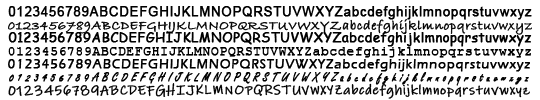
\includegraphics[width=8cm]{update-fig-dataset.png}

    Figure 2. The dataset currently used in training.\\The first line is extracted from the Arial font and\\is used as the base font described in the next section.
\end{center}
The dataset is generated by a render module which can extract images of specific characters from True Type font files, and devided into train, validation and test sets by the ratio of 8:1:1 randomly.


\section{Model}
We built a Generative Adversarial Network, which consists of a generator and a 5-layer discriminator. Since the end-to-end StyleGAN generator did not meet our expectations after preliminary training, we tried two other generators. The following subsections will introduce them in turn.

\subsection{End-to-end StyleGAN Generator}
This is the generator model what we first envisaged, which is modified from the basic StyleGAN generator. The original full-connected mapping network is replaced by an convolutional network to extract style information directly from input images.
\\
\begin{center}
    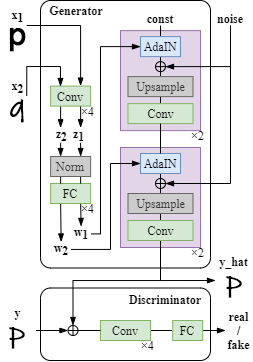
\includegraphics[]{update-fig-model.png}

    Figure 3. Rough structure of our end-to-end StyleGAN\\generator and discriminator. The generator includes a\\4-layerCNN encoder, a 4-layer Mapping Network and a\\4-layer Synthesis Network(CNN decoder with AdaIN).
\end{center}
On each training epoch, two images of different fonts are fed into the downscaling network on the left to produce intermediate vectors $w_1$ and $w_2$. In the upsacling network on the right, the one providing the skeleton will be used for the lower part of the decoder, and the one providing the style will be used for the upper part.
\\
Denote an image of character $i$ and font $F_k$ by $F_k[i]$. For each time, the generator takes a pair of images $(x_1=F_0[i], x_2=F_k[j])$ and outputs an image $\hat{y}$ with skeleton of $x_1$ and style of $x_2$. The discriminator differs the output from the groundtruth image $y=F_k[i]$. Font $F_0$ is the base font, which should have clear skeletons, and can be the same whenever training or testing.

\subsection{U-Net Generator}
We also built a traditional pix2pix U-Net Generator with 4 downscaling blocks and 4 upscaling blocks. The inputs and outputs are the same with previous end-to-end StyleGAN Generator, where $x_1$ and $x_2$ are concatenated in the channel dimention and input to the first downscaling block as a whole $32 \times 32 \times 2$ image.
\\
In order to make the model converge in the early stage, we added a $l1$-loss term to the generator's loss function.

\subsection{Original Latent-based StyleGAN Generator with Pre-trained latent encoder}
Due to the end-to-end StyleGAN generator is hard to converge in training, we turned back to the origin latent-based StyleGAN generator which inputs gaussian distributed latents to the mapping network. To perform style-mixing, we can input different latents at different layers while evaluating and testing.
\\
Unlike most cases, we can not simply generate random gaussian latents to train the model. Instead, we need a well-trained latent encoder to deal with new inputs.
This step is something we haven't done yet, and we're going to pre-train a CNN autoencoder to extract latent from images.


\section{Training}
We followed the basic GAN training process:
\smallskip \noindent
\\
\hspace*{3mm} For epoch in epochs\\
\hspace*{6mm} For iteration in iterations\\
\hspace*{9mm} Get next training data\\
\hspace*{9mm} Forward Generator\\
\hspace*{9mm} Forward Discriminator\\
\hspace*{9mm} Freeze gradients of Generator\\
\hspace*{9mm} Backward and optimize Discriminator\\
\hspace*{9mm} Freeze gradients of Discriminator\\
\hspace*{9mm} Backward and optimize Generator\\
\hspace*{3mm} Run evaluation\\
\\
\smallskip \noindent
Here are the adjustable hyperparameters during training process:
\begin{table}[h]
    \centering
    \begin{tabular}{|l|c|}
        \hline
        Hyperparameter&Default Value\\
        \hline
        Epoch Number&100\\
        Iteration Number&2000\\
        Batch Size&8\\
        Optimizer&Adam\\
        Learning Rate&0.01\\
        GAN loss&Least Squares\\
        \hline
    \end{tabular}
    \caption{Hyperparameters for GAN}
\end{table}

\subsection{End-to-end StyleGAN Generator}
\begin{table}[h]
    \centering
    \begin{tabular}{|l|c|}
        \hline
        Hyperparameter&Default Value\\
        \hline
        Mapping Network Layers&4\\
        Synthesis Network Layers&4\\
        Interval Vector Size&512\\
        Add Noise&None\\
        \hline
    \end{tabular}
    \caption{Hyperparameters for GAN}
\end{table}

\subsection{U-Net}
\begin{table}[h]
    \centering
    \begin{tabular}{|l|c|}
        \hline
        Hyperparameter&Default Value\\
        \hline
        Downscaling Layers&4\\
        Upscaling Layers&4\\
        L1 loss weight&10\\
        G/D Training Ratio&10\\
        \hline
    \end{tabular}
    \caption{Hyperparameters for GAN}
\end{table}

\subsection{Original StyleGAN Generator}
\begin{table}[h]
    \centering
    \begin{tabular}{|l|c|}
        \hline
        Hyperparameter&Default Value\\
        \hline
        Mapping Network Layers&4\\
        Synthesis Network Layers&4\\
        Input Latent Size&512\\
        Interval Vector Size&512\\
        Add Noise&None\\
        \hline
    \end{tabular}
    \caption{Hyperparameters for GAN}
\end{table}

\subsection{Hyperparameter Selection on U-Net}
We decided to change 1 hyperparameter a time which are 6 models totally. The measurement of these models are the mse loss of $y$ and $\hat{y}$ we generate. We compute the loss every epoch for validation dataset. Here is a figure of the loss per sample among epochs.

\begin{center}
    \includegraphics[width=.5\textwidth]{./update-figs/MSE loss among epochs.png}

    Figure 4. MSE Loss among epochs for 6 different models.
\end{center}

From this figure, we found that using lsgan loss funtion could make the model perform better. And for only lsgan models, we have plot them in a separate figure shown below. In this figure, we observed when learning rate is enlarge to 0.03, the model performs better, and when $gdrate$ is reduced to 1, the model perform worst. Since the default setting is the second best, we believe the hyperparameters $lr=0.03$, $batchsize=8$, $gdrate=10$ and $GAN loss=lsgan$ is a fairly good parameter setting.

\begin{center}
    \includegraphics[width=.5\textwidth]{./update-figs/MSE loss among epochs without wgan.png}

    Figure 5. MSE Loss among epochs without wgan for 5 different models.
\end{center}

It should be noted that the MSE loss is not always declining. There may be two reasons:

\begin{itemize}
    \item The MSE loss function is not a good measure of image similarity. After the generator learns to generate images with appropriate brightness, MSE can no longer measure how close $\hat{y}$ and $y$ are
    \item The training process after several epochs is doing useless work. The L1 loss's guidance becomes useless or even wrong, or we have hit the upper limit of the model.
\end{itemize}


\section{Preliminary Results}
\subsection{End-to-end StyleGAN Generator}
As we mentioned before, our end-to-end StyleGAN Generator does not converges during the training process.

\begin{center}
    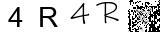
\includegraphics[width=.2\textwidth]{./update-figs/e2estylegan_1.jpg}
    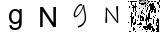
\includegraphics[width=.2\textwidth]{./update-figs/e2estylegan_2.jpg}\\
    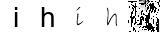
\includegraphics[width=.2\textwidth]{./update-figs/e2estylegan_3.jpg}
    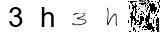
\includegraphics[width=.2\textwidth]{./update-figs/e2estylegan_4.jpg}\\
    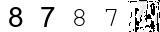
\includegraphics[width=.2\textwidth]{./update-figs/e2estylegan_5.jpg}
    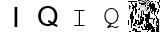
\includegraphics[width=.2\textwidth]{./update-figs/e2estylegan_6.jpg}\\

    Figure 6. A typical test output of our end-to-end\\StyleGAN generator. From left to right:\\$x_0=F_0[i]$ (not as input), $x_1=F_0[j]$,\\$x_2=F_k[i]$, $y=F_k[j]$, $\hat{y}=G(x_1,x_2)$
\end{center}

\subsection{U-Net Generator}
Here are several outputs sampled from the test result of U-Net generator with minimum MSE loss. 

\begin{center}
    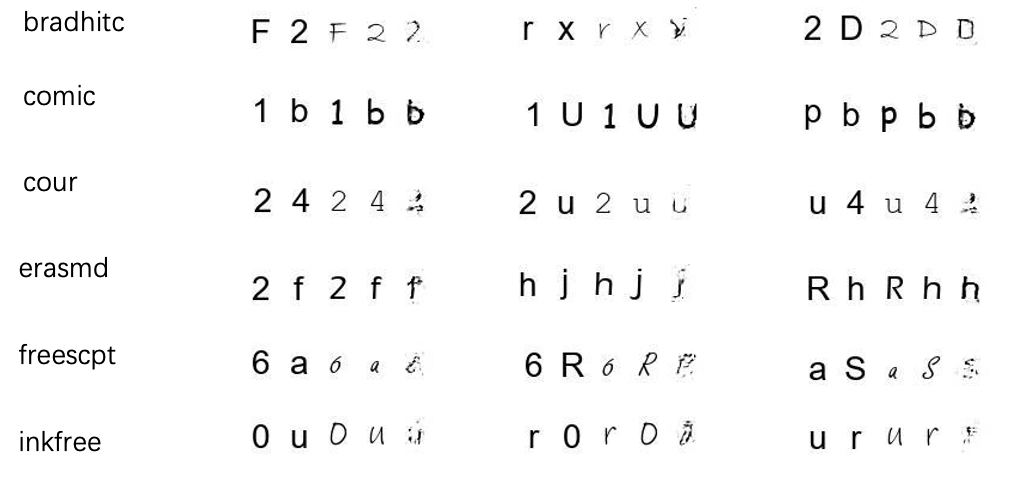
\includegraphics[width=.5\textwidth]{./update-figs/lr_0.03_batchsize_8_g_d_rate_10_loss_lsgan.png}

    Figure 7. U-Net results under $lr=0.03$, $batchsize=8$, $gdrate=10$ and $GAN loss=lsgan$.
\end{center}

It can be seen that the U-Net model has initially possessed the ability of style transfer.

\subsection{Original Latent-based StyleGAN Generator}
Since we have not completed the training of autoencoder, we can only train the original latent-based StyleGAN generator with randomly generated gaussian latents at present. Here are several sample outputs generated by  the generator after 10 epoches training.

\begin{center}
    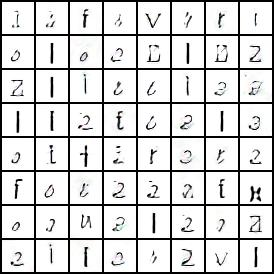
\includegraphics[width=.3\textwidth]{./update-figs/latentstylegan.jpg}

    Figure 8. Results of original latent-based StyleGAN generator trained with random gaussian latents.
\end{center}

The original StyleGAN generator can quickly fit the dataset and generate character images. However, whether it can successfully transfer the style of a new image still depends on the training results of the autoencoder.

\section{Remaining Works and Concerns}
\subsection{End-to-end StyleGAN Generator}
\begin{itemize}
    \item The current CNN mapping network may not be able to extract style latents efficiently. We are designing a new one.
    \item The training process we implemented may have errors in details. We intend to re-read the open-source StyleGAN code carefully to make sure our implementation is right.
    \item We already know that direct training with two input images is not convergent. We are trying to introduce some early training tricks.
    \item The CNN encoder block is shared by two independent datapaths and provides relatively more static functions, which means it can be pre-trained rather than roughly training the whole generator together.
\end{itemize}

\subsection{U-Net Generator}
\begin{itemize}
    \item From the trend diagram of MSE loss, we can see that there is no large performance improvement after the first few epochs. We may need new loss functions and training tricks to further improve the U-Net generator.
    \item The network structure can be simplified. According to our previous assumptions, the high-level blocks control the style and the low-level blocks control the skeleton, We can observe the parameters of the current model and selectively cut off some connections with low utilization.
\end{itemize}

\subsection{End-to-end StyleGAN generator}
\begin{itemize}
    \item The autoencoder is not so easy to design and train. What we want is a network that can encode and decode images of any font and any characters. To achieve this goal, the current data set may not be enough.
    \item Because it is not an end-to-end epproach, the quality of style mixing is uncontrollable. To be specific, we may not be able to use $y=F_k[j]$ to guide the generator to improve the style mixing result.
\end{itemize}

\section{Reference}
\smallskip \noindent
Leon, A. G., Alexander, S. E., and Matthias, B. 2016. Image Style Transfer Using Convolutional Neural Networks. \textit{CVPR}, pp. 2414-2423.

\smallskip \noindent
Tero, K., Samuli, L., and Timo, A. 2019. A Style-Based Generator Architecture for Generative Adversarial Networks. \textit{CVPR}, abs/1812.04948.

\smallskip \noindent
Ko, D. H., Hassan, A. U., Suk, J., \& Choi, J. 2021. SKFont: skeleton-driven Korean font generator with conditional deep adversarial networks. \textit{International Journal on Document Analysis and Recognition (IJDAR)}, 1-13.

\smallskip \noindent
Bhunia, A. K., Bhunia, A. K., Banerjee, P., Konwer, A., Bhowmick, A., Roy, P. P., \& Pal, U. 2018. Word level font-to-font image translation using convolutional recurrent generative adversarial networks. \textit{ICPR} (pp. 3645-3650).


\section{Appendix}
Our code repository: https://github.com/Starmys/FontStyleTransfer

\bibliography{proposal-reference.bib}
\bibliographystyle{aaai}
\end{document}